\documentclass[handout]{ximera}
%handout:  for handout version with no solutions or instructor notes
%handout,instructornotes:  for instructor version with just problems and notes, no solutions
%noinstructornotes:  shows only problem and solutions

%% handout
%% space
%% newpage
%% numbers
%% nooutcomes

%I added the commands here so that I would't have to keep looking them up
%\newcommand{\RR}{\mathbb R}
%\renewcommand{\d}{\,d}
%\newcommand{\dd}[2][]{\frac{d #1}{d #2}}
%\renewcommand{\l}{\ell}
%\newcommand{\ddx}{\frac{d}{dx}}
%\everymath{\displaystyle}
%\newcommand{\dfn}{\textbf}
%\newcommand{\eval}[1]{\bigg[ #1 \bigg]}

%\begin{image}
%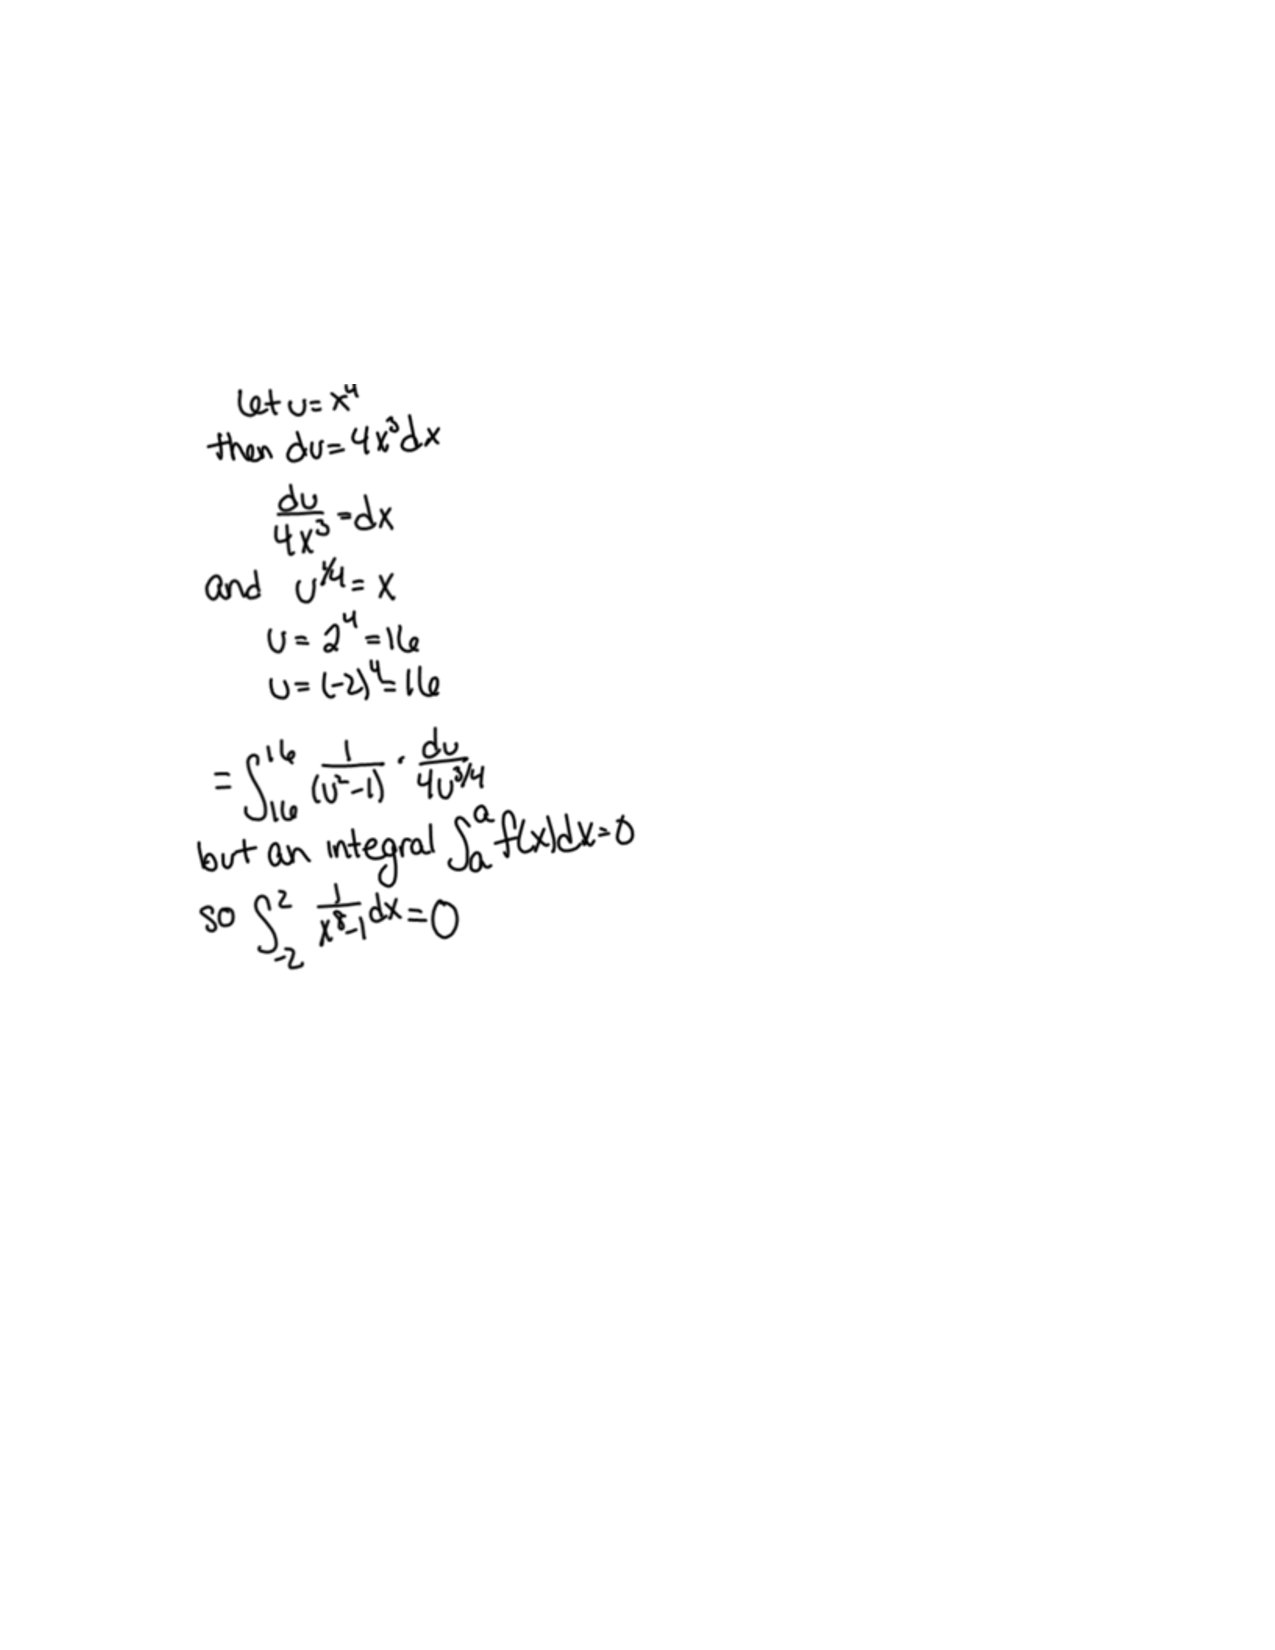
\includegraphics[trim= 170 420 250 180]{Figure1.pdf}
%\end{image}

%add a ``.'' below when used in a specific directory.
\newcommand{\RR}{\mathbb R}
\renewcommand{\d}{\,d}
\newcommand{\dd}[2][]{\frac{d #1}{d #2}}
\renewcommand{\l}{\ell}
\newcommand{\ddx}{\frac{d}{dx}}
\newcommand{\dfn}{\textbf}
\newcommand{\eval}[1]{\bigg[ #1 \bigg]}

\usepackage{multicol}

\renewenvironment{freeResponse}{
\ifhandout\setbox0\vbox\bgroup\else
\begin{trivlist}\item[\hskip \labelsep\bfseries Solution:\hspace{2ex}]
\fi}
{\ifhandout\egroup\else
\end{trivlist}
\fi} %% we can turn off input when making a master document

\title{Recitation \#15: Sequences and Infinite Series}  

\begin{document}
\begin{abstract}		\end{abstract}
\maketitle



\section{Warm up:}
Find the limit of the following sequences as $n$ tends to $\infty$. 
\begin{enumerate}

\item $a_n = \frac{n^{1000}}{2^n}$

	
\item $b_n = \cos (n \pi)$

\item $c_n = \cos (n! \pi)$

\end{enumerate}
	\begin{freeResponse}
\begin{enumerate}	
\item Note that $\lim_{x \to \infty} \frac{x^a}{b^x} = 0$ for any constants $a$ and $b>1$. So $\lim_{n \to \infty} a_n =0$.
\item If $n$ is even, $b_n = \cos(n \pi) = 1$, but if $n$ is odd, then $b_n = \cos(n \pi) = -1$. So $\lim_{n \to \infty} b_n$ does not exist.
\item If $n$ is at least 2, then $n!$ is even. So $c_n = 1$ if $n$ is at least 2. $\lim_{n \to \infty} c_n = 1$. 
\end{enumerate}
	\end{freeResponse}
\begin{instructorNotes}

\end{instructorNotes}







\section{Group work:}



%problem 1
\begin{problem}
For each of the following sequences, find the limit as the number of terms approaches infinity.
	\begin{enumerate}
	
	\item  $a_n = \left( \frac{n+1}{2n} \right) \left( \frac{n-2}{n} \right)^{\frac{n}{2}}$
	\begin{freeResponse}
	Let $f(x) =  \left( \frac{x+1}{2x} \right) \left( \frac{x-2}{x} \right)^{\frac{x}{2}}$.  
	Then
		\begin{align*}
		\lim_{x \to \infty} f(x) 
		&= \lim_{x \to \infty} e^{\ln f(x)}  \\
		&= e^{\lim_{x \to \infty} \ln f(x)}.
		\end{align*}
	So we need to compute the limit in the exponent.  To this end
		\begin{align*}
		\lim_{x \to \infty} \ln f(x) 
		&= \lim_{x \to \infty} \left[ \ln \left( \frac{x+1}{2x} \right) + \ln \left( \frac{x-2}{x} \right)^{\frac{x}{2}} \right]  \\
		&= \lim_{x \to \infty} \ln \left( \frac{x+1}{2x} \right) + \lim_{x \to \infty} \left[ \frac{x}{2} \ln \left( \frac{x-2}{x} \right) \right]  \quad {\color{red}\text{provided both limits exist}}  \\
		&= \ln \left( \frac{1}{2} \right) + \lim_{x \to \infty} \frac{\ln \left( 1 - \frac{2}{x} \right)}{\frac{2}{x}}  \quad {\color{red}\text{indeterminant of the form }\frac{0}{0}}\\
		&= \ln \left( \frac{1}{2} \right) + \lim_{x \to \infty} \frac{\frac{2x^{-2}}{1-\frac{2}{x}}}{-2x^{-2}}  \quad {\color{red}\text{L'Hospital's Rule}}  \\
		&= \ln \left( \frac{1}{2} \right) + \lim_{x \to \infty} \frac{-1}{1-\frac{2}{x}}  \\
		&= \ln \left( \frac{1}{2} \right) - 1.
		\end{align*}
	So 
		\[
		\lim_{x \to \infty} f(x) = e^{\ln \left( \frac{1}{2} \right) - 1} = \frac{1}{2} e^{-1}
		\]
	and therefore
		\[
		\lim_{n \to \infty} \left( \frac{n+1}{2n} \right) \left( \frac{n-2}{n} \right)^{\frac{n}{2}} = \frac{1}{2} e^{-1}.
		\]
	\end{freeResponse}
	
	
	
	\item  $a_n = \sqrt[n]{3^{2n+1}}$
	\begin{freeResponse}
		\begin{align*}
		\lim_{n \to \infty} \sqrt[n]{3^{2n+1}}
		&= \lim_{n \to \infty} \left( 3^{2n+1} \right)^{\frac{1}{n}}  \\
		&= \lim_{n \to \infty} 3^{2 + \frac{1}{n}}  \\
		&= \lim_{n \to \infty} 3^2 \cdot 3^{\frac{1}{n}}  \\
		&= 9 \lim_{n \to \infty} e^{\frac{1}{n}}  \\
		&= 9 \cdot 3^0  \\
		&= 9 \cdot 1 = 9.
		\end{align*}
	\end{freeResponse}
	
	
	
	\item  $a_n = \left( \sqrt{n^2+7} - n \right)$
	\begin{freeResponse}
		\begin{align*}
		\lim_{n \to \infty} \left( \sqrt{n^2+7} - n \right)
		&= \lim_{n \to \infty} \left[ \left( \sqrt{n^2 + 7} - n \right) \cdot \frac{\sqrt{n^2 + 7} + n}{\sqrt{n^2 + 7} + n} \right]  \\
		&= \lim_{n \to \infty} \frac{n^2 + 7 - n^2}{n \sqrt{1 + \frac{7}{n^2}} + n}  \\
		&= \lim_{n \to \infty} \frac{7}{n ( \sqrt{1 + \frac{7}{n^2}} + 1)}  \\
		&= 0.
		\end{align*}
	\end{freeResponse}
	
	
	
	\item  $a_n = \frac{(2n+3)!}{5n^3 (2n)!}$
	\begin{freeResponse}
		\begin{align*}
		\lim_{n \to \infty} \frac{(2n+3)!}{5n^3(2n)!}
		&= \lim_{n \to \infty} \frac{(2n+3)(2n+2)(2n+1)(2n)!}{5n^3(2n)!}  \\
		&= \lim_{n \to \infty} \frac{(2n+3)(2n+2)(2n+1)}{5n^3}  \\
		&= \frac{8}{5} 	\quad	{\color{red}\text{Compare the coefficients of the leading }n^3 \text{terms}}
		\end{align*}
	\end{freeResponse}
	
	
	
	\item  $a_n = (2^n + 3^n)^{\frac{1}{n}}$  
	\begin{center}
	{\it Hint:  $a_n \geq (0+3^n)^{\frac{1}{n}} = 3$ and $a_n \leq (2 \cdot 3^n)^{\frac{1}{n}} = 2^{\frac{1}{n}} \cdot 3$}
	\end{center}
	\begin{freeResponse}
	From the hint
		\[
		3 = (0+3^n)^\frac{1}{n}  \leq a_n \leq (2 \cdot 3^n)^\frac{1}{n} = 2^\frac{1}{n} \cdot 3.
		\]
	So by the squeeze theorem, we have that
		\begin{align*}
		\lim_{n \to \infty} 3 \leq &\lim_{n \to \infty} a_n \leq \lim_{n \to \infty} 2^\frac{1}{n} \cdot 3  \\
		\Longrightarrow 	\qquad	3 \leq &\lim_{n \to \infty} a_n \leq 1 \cdot 3 = 3.
		\end{align*}
	Thus,
		\[
		\lim_{n \to \infty} a_n = 3.
		\]
	\end{freeResponse}
	
	
	
	\item  $a_n = \frac{n^{365} + 5^n}{8^n + n^3}$
	\begin{freeResponse}
		\begin{align*}
		\lim_{n \to \infty} \frac{n^{365} + 5^n}{8^n + n^3}
		&= \lim_{n \to \infty} \frac{n^{365} + 5^n}{8^n + n^3} \cdot \frac{\frac{1}{8^n}}{\frac{1}{8^n}}  \\
		&=  \lim_{n \to \infty} \frac{\frac{n^{365}}{8^n} + \left( \frac{5}{8} \right)^n}{1 + \frac{n^3}{8^n}}  \\
		&= \frac{0+0}{1+0} = 0.		\quad	{\color{red}\text{due to growth rates,} \lim_{n \to \infty} \frac{n^k}{a^n} = 0.}
		\end{align*}
	\end{freeResponse}
	
	

	
	\end{enumerate}
	
\end{problem}

\begin{instructorNotes}
For this problem, give each group two of the problems to report on.  
Give about $8$ minutes (or less?) for the group work and about $10-15$ minutes for discussion.  
On (a), L'Hospital's Rule is involved.  
On (e), the squeeze theorem should be involved.  
On (f), the students may use ``known'' facts of the relative growth of polynomial vs. exponential terms.
\end{instructorNotes}







%problem 2
\begin{problem}
Show that 
$$\lim_{n \to \infty} \left( \sqrt{n+1} - \sqrt{n} \right)$$ 
exists by proving that $a_n = \sqrt{n+1} - \sqrt{n}$ is a bounded monotonic sequence.  A hint is to show that $f(x) = \sqrt{x+1} - \sqrt{x}$ is a decreasing function by showing that $f'(x) < 0$.  
	\begin{freeResponse}
	Let $f(x) = \sqrt{x+1} - \sqrt{x}$.  Then
		\begin{align*}
		f'(x) 
		&= \frac{1}{2 \sqrt{x+1}} - \frac{1}{2 \sqrt{x}}  \\
		&= \frac{\sqrt{x} - \sqrt{x+1}}{2 \sqrt{x}\sqrt{x+1}}  \\
		&< 0
		\end{align*}
	since the denominator is clearly positive, and $\sqrt{x} < \sqrt{x+1}$.
	Therefore $f$ is decreasing, and so the original sequence is decreasing.  
	Also notice that since 
	$$\sqrt{x} < \sqrt{x+1}$$
	we have that 
	$$0 < \sqrt{x+1} - \sqrt{x} = f(x).$$
	Thus the original sequence is bounded below by $0$.  \

	Therefore, since the sequence $\left\{ \sqrt{n+1} - \sqrt{n} \right\}$ is bounded and monotone decreasing, the limit
		\[
		\lim_{n \to \infty} \sqrt{n+1} - \sqrt{n}
		\]
	exists.
	\end{freeResponse}
		
\end{problem}

\begin{instructorNotes}
Perhaps do as a whole class discussion.  
Emphasize careful writing of reasoning.
\end{instructorNotes}







%problem 3
\begin{problem}
Find the limit of the given sequence.  
Also, determine if it is a geometric sequence.
	\begin{multicols}{3}
	\begin{enumerate}
	
	\item  $a_n = \frac{n^2}{2^n}$
	%\begin{freeResponse}
	
	%\end{freeResponse}
	
	
	
	\item  $a_n = \frac{1}{3^n}$
	%\begin{freeResponse}
	
	%\end{freeResponse}
	
	
	
	\item  $a_n = \left( \frac{1}{n} \right)^4$
	%\begin{freeResponse}
	
	%\end{freeResponse}
	
	
	
	\item  $a_n = \frac{e^n + (-3)^n}{5^n}$
	%\begin{freeResponse}
	
	%\end{freeResponse}
	
	
	
	\item  $a_n = 3^{\frac{1}{n}}$
	%\begin{freeResponse}
	
	%\end{freeResponse}
	
	\end{enumerate}
	\end{multicols}
	
	\begin{freeResponse}
	\begin{enumerate}
	\item 	$\lim_{n \to \infty} \frac{n^2}{2^n} = 0 	\quad	{\color{red}\text{growth rate}}$
	
	\item  $\lim_{n \to \infty} \frac{1}{3^n} = \lim_{n \to \infty} \left( \frac{1}{3} \right)^n = 0.$
	This is a geometric sequence with $a = 1$ and $r = \frac{1}{3}$.  
	
	\item  $\lim_{n \to \infty} \left( \frac{1}{n} \right)^4 = 0$.  
	
	\item  $\lim_{n \to \infty} \frac{e^n + (-3)^n}{5^n} = \lim_{n \to \infty} \left[ \left( \frac{e}{5} \right)^n + \left( \frac{-3}{5} \right)^n \right] = 0.$  
	
	This is the sum of two geometric sequences.  
	For both, the initial term is $a = 1$.  
	For the first sequence the ratio is $r_1 = \frac{e}{5}$, and for the second the ratio is $r_2 = \frac{-3}{5}$.
	
	\item  $\lim_{n \to \infty} 3^\frac{1}{n} = 3^0 = 1$.  
	
	\end{enumerate}
	\end{freeResponse}

\end{problem}

\begin{instructorNotes}
These limits should be relatively easy to analyze.  
The students need to identify the ``$r$'' if it is a geometric sequence (and note that the exponent $n$ is the variable).  
On (d) and (f), they should argue that they are looking at the sum of two geometric sequences.  
Maybe give one per group with about $8$ minutes for discussion.  
\end{instructorNotes}







\begin{problem}
Determine if the following series converge or diverge.  If they converge, find the sum.
	\begin{enumerate}
	
	\item  $e + 1 + e^{-1} + e^{-2} + e^{-3} + \hdots$
	\begin{freeResponse}
		\begin{align*}
		e + 1 + e^{-1} + e^{-2} + e^{-3} + \hdots
		&= e + \sum_{k = 0}^\infty e^{-k}  \\
		&= e + \sum_{k=0}^\infty \left( e^{-1} \right)^k 	\quad	{\color{red}\text{geometric series, }r = e^{-1} < 1}  \\
		&= e + \frac{1}{1-e^{-1}}.
		\end{align*}
	Therefore, this series converges to $\left( e + \frac{1}{1-e^{-1}} \right)$.  
	\end{freeResponse}
	
	
	
	\item  $\sum_{k=0}^{99} 2^k + \sum_{k=100}^\infty \frac{1}{2^k}$
	\begin{freeResponse}
	Let us analyze the two different summands in this problem:
		\begin{enumerate}
		\item[(i)]  $\sum_{k=0}^{99} 2^k$
		
		This is a finite sum from a geometric sequence, and so its sum is 
			\[
			\frac{a(1-r^n)}{1-r}.
			\]
		Thus,
	  		\[
	  		\sum_{k=0}^{99} 2^k = \frac{1(1-2^{100})}{1-2} = 2^{100} - 1.
	  		\]
	  		
		\item[(ii)]  $\sum_{k=100}^\infty \frac{1}{2^k} = \sum_{k=100}^\infty \left( \frac{1}{2} \right)^k$.  
		
		This is a geometric series with $a=\frac{1}{2^{100}}$ and $r = \frac{1}{2}$.  
		So
			\[
			\sum_{k=100}^\infty \frac{1}{2^k} = \frac{\frac{1}{2^{100}}}{1-\frac{1}{2}} = \frac{1}{2^{99}}.
			\]
			
	Therefore, combining parts (i) and (ii) we have that
		\[
		\sum_{k=0}^{99} 2^k + \sum_{k=100}^\infty \frac{1}{2^k} = 2^{100} - 1 + \frac{1}{2^{99}}.
		\]
		\end{enumerate}
	\end{freeResponse}
	
	
	
	\item  $\sum_{k=0}^\infty (\cos(1))^k$
	\begin{freeResponse}
	This is a geometric series with $a=1$ and $r = \cos(1)$.  
	We know that $-1 < \cos(1) < 1$, and so $|\cos(1)|<1$.  
	Therefore, this geometric series converges and
		\begin{align*}
		\sum_{k=0}^\infty (\cos(1))^k = \frac{1}{1-\cos(1)}.
		\end{align*}
	\end{freeResponse}
	
	
	
	\item  $\sum_{k=4}^\infty \frac{5 \cdot 4^{k+3}}{7^{k-2}}$
	\begin{freeResponse}
	Let us first reindex this series.  
	Let $\ell = k-4$.  
	Then $k=\ell+4$, and when $k=4$, $\ell = 0$.
	We then have that
		\begin{align*}
		\sum_{k=4}^\infty \frac{5 \cdot 4^{k+3}}{7^{k-2}}
		&= \sum_{\ell=0}^\infty \frac{5 \cdot 4^{\ell + 4 + 3}}{7^{\ell + 4 - 2}}  \\
		&= \sum_{\ell=0}^\infty \frac{5 \cdot 4^{\ell + 7}}{7^{\ell + 2}}  \\
		&= \sum_{\ell=0}^\infty \frac{5 \cdot 4^7 \cdot 4^\ell}{7^2 \cdot 7^\ell}  \\
		&= \frac{5 \cdot 4^7}{7^2} \sum_{\ell=0}^\infty \left( \frac{4}{7} \right)^\ell  \quad	{\color{red}\text{assuming this series converges}}  \\
		&= \frac{5 \cdot 4^7}{7^2} \cdot \frac{1}{1-\frac{4}{7}}  \quad  {\color{red}\text{geometric series with }a=1, r = \frac{4}{7}}  \\
		&= \frac{5 \cdot 4^7}{3 \cdot 7}.
		\end{align*}
	Therefore, this series converges to $\frac{5 \cdot 4^7}{3 \cdot 7}$.  
	\end{freeResponse}
	
	
	
	\item  $\sum_{k=0}^\infty e^{5-2k}$
	\begin{freeResponse}
		\begin{align*}
		\sum_{k=0}^\infty e^{5-2k}
		&= \sum_{k=0}^\infty \left[ e^5 \cdot \left( e^{-2} \right)^k \right]  \\
		&= e^5 \sum_{k=0}^\infty \left( e^{-2} \right)^k  	\quad	{\color{red}\text{assuming the series converges}}  \\
		&= e^5 \cdot \frac{1}{1-e^{-2}}  \quad 	{\color{red}\text{geometric series with }a=1, r=e^{-2} < 1}
		\end{align*}
	Therefore, this series converges to $\frac{e^5}{1-e^{-2}}$.  
	\end{freeResponse}
	
	
	
	\item  $\sum_{k=0}^\infty \frac{e^k + (-7)^k}{5^k}$
	\begin{freeResponse}
		\begin{align*}
		\sum_{k=0}^\infty \frac{e^k + (-7)^k}{5^k} 
		&= \sum_{k=0}^\infty \left[ \frac{e^k}{5^k} + \frac{(-7)^k}{5^k} \right]  \\
		&= \sum_{k=0}^\infty \left[ \left( \frac{e}{5} \right)^k + \left( \frac{-7}{5} \right)^k \right] . \\
		\end{align*}
	If both of these series were convergent, then we would be able to split up the sum:
		\[  
		\sum_{k=0}^\infty \frac{e^k + (-7)^k}{5^k} ``=" \sum_{k=0}^\infty \left( \frac{e}{5} \right)^k + \sum_{k=0}^\infty \left( \frac{-7}{5} \right)^k.
		\]
	The first series on the right hand side is a geometric series with $r=\frac{e}{5}$.  
	Since $\biggr| \frac{e}{5} \biggr| < 1$, this series converges.  
	But the second series is a geometric series with $r = \frac{-7}{5}$.  
	Since $\biggr| \frac{-7}{5} \biggr| > 1$, this series diverges.
	
	Therefore, the original series diverges.
	\end{freeResponse}
	
	
	
	\item  $ \sum_{k=0}^\infty \left[ \frac{5}{(k+1)(k+2)} + \left( - \frac{1}{2} \right)^k \right]$
	\begin{freeResponse}
	If both series converge, then we can break up the sum:
		\[
		\sum_{k=0}^\infty \left[ \frac{5}{(k+1)(k+2)} + \left( - \frac{1}{2} \right)^k \right] = \sum_{k=0}^\infty \frac{5}{(k+1)(k+2)} + \sum_{k=0}^\infty \left( - \frac{1}{2} \right)^k.
		\]
	Let us consider both series on the right hand side of this equation individually.
		\begin{enumerate}
		\item[(i)]  $\sum_{k=0}^\infty \left( - \frac{1}{2} \right)^k$
		
		This is a geometric series with $a=1$ and $r = \frac{-1}{2}$.  
		Therefore, this series converges with
			\[
			\sum_{k=0}^\infty \left( - \frac{1}{2} \right)^k = \frac{1}{1- \left( \frac{-1}{2} \right)}  = \frac{2}{3}.
			\]
		
		\item[(ii)]  $\sum_{k=0}^\infty \frac{5}{(k+1)(k+2)}$
		
		It may not be obvious yet, but this is a telescoping series.  
	To see this, let us decompose $\frac{5}{(k+1)(k+2)}$ as a partial fraction.
		\begin{align*}
		&\frac{5}{(k+1)(k+2)} = \frac{A}{k+1} + \frac{B}{k+2}  \\
		\Longrightarrow 	\qquad 	&5 = A(k+2) + B(k+1).
		\end{align*}
	We solve for $A$ and $B$ by choosing ``smart" values for $k$:
		\begin{align*}
		&(k=-1) 	\quad	\Longrightarrow 	\quad	A = 5  \\
		&(k=-2) 	\quad	\Longrightarrow		\quad	-B = 5 	\quad	\Longrightarrow		\quad	B = -5.
		\end{align*}
	So we see that
		\begin{align*}
		\sum_{i=1}^\infty \left( \frac{1}{i} - \frac{1}{i+2} \right) = \sum_{k=0}^\infty \left[ \frac{5}{k+1} - \frac{5}{k+2} \right].
		\end{align*}
	Let 
		\[
		S_n = \sum_{k=0}^n \left[ \frac{5}{k+1} - \frac{5}{k+2} \right].
		\]
	Then we have that
		\begin{align*}
		S_n &= \sum_{k=0}^n \left[ \frac{5}{k+1} - \frac{5}{k+2} \right]  \\
		&= \left( \frac{5}{1} - \frac{5}{2} \right) + \left( \frac{5}{2} - \frac{5}{3} \right) + \left( \frac{5}{3} - \frac{5}{4} \right) + \hdots + \left( \frac{5}{n+1} - \frac{5}{n+2} \right)  \\
		&= \frac{5}{1} - \frac{5}{n+2} = 5 - \frac{5}{n+2}.
		\end{align*}
	We then compute the sum by taking the limit of the sequence of partial sums:
		\begin{align*}
		\sum_{k=0}^\infty \frac{5}{(k+1)(k+2)}
		&= \lim_{n \to \infty} \sum_{k=0}^n \frac{5}{(k+1)(k+2)}  \\
		&= \lim_{n \to \infty} S_n  \\
		&= \lim_{n \to \infty} \left( 5 - \frac{5}{n+2} \right)  \\
		&= 5.
		\end{align*}
		\end{enumerate}
	\vskip 5pt
	Finally, we compute the sum of the original series as
		\begin{align*}
		\sum_{k=0}^\infty \left[ \frac{5}{(k+1)(k+2)} + \left( - \frac{1}{2} \right)^k \right] 
		&= \sum_{k=0}^\infty \frac{5}{(k+1)(k+2)} + \sum_{k=0}^\infty \left( - \frac{1}{2} \right)^k  \\
		&= 5 + \frac{2}{3} = \frac{17}{3}.
		\end{align*}
	\end{freeResponse}
	
	
	
	\item  $\sum_{i=1}^\infty \left( \frac{1}{i} - \frac{1}{i+2} \right)$
	
	\begin{freeResponse}
	This is a telescoping series.  
	Let 
		\[
		S_n = \sum_{i=1}^n \left( \frac{1}{i} - \frac{1}{i+2} \right).
		\]
	Then,
		\begin{align*}
		S_n &= \sum_{i=1}^n \left( \frac{1}{i} - \frac{1}{i+2} \right)  \\
		&= \left( {\color{red}\frac{1}{1}} - \frac{1}{3} \right) + \left( {\color{red}\frac{1}{2}} - \frac{1}{4} \right) + \left( \frac{1}{3} - \frac{1}{5} \right) + \left( \frac{1}{4} - \frac{1}{6} \right) + \left( \frac{1}{5} - \frac{1}{7} \right)  \\
		&+ \hdots + \left( \frac{1}{n-2} - \frac{1}{n} \right) + \left( \frac{1}{n-1} - {\color{red}\frac{1}{n+1}} \right) + \left( \frac{1}{n} - {\color{red}\frac{1}{n+2}} \right)  \\
		&= 1 + \frac{1}{2} - \frac{1}{n+1} - \frac{1}{n+2}.
		\end{align*}
	Note that the last equality above is because all of the non-red terms cancel (convince yourself of this).  
	Then
		\begin{align*}
		\sum_{i=1}^\infty \left( \frac{1}{i} - \frac{1}{i+2} \right)
		&= \lim_{n \to \infty} S_n  \\
		&= \lim_{n \to \infty} \left[ 1 + \frac{1}{2} - \frac{1}{n+1} - \frac{1}{n+2} \right]  \\
		&= 1 + \frac{1}{2} = \frac{3}{2}.
		\end{align*}
	\end{freeResponse}
	
	\end{enumerate}
	
\end{problem}

\begin{instructorNotes}
Assign two per group.  
Most of these involve geometric series and one (part (b)) involves a finite geometric sum, whose ``trick'' is presented in the lecture.  

Students must identify the ``$r$'' and pay attention to both the indices and the exponents (for example, $7^{k+3} = 7^3 \cdot 7^k$).  
Encourage multiple methods (there are $3$ methods presented in the lecture) and make sure students clearly explain their reasoning on paper.  
\end{instructorNotes}







%problem 2
\begin{problem}
Convert the decimal $2.456\overline{314}$ to a fraction using geometric series.
	\begin{freeResponse}
		\begin{align*}
		2.456\overline{314}
		&= 2.456 + 0.000314 + 0.000000314 + \hdots  \\
		&= 2.456 + \frac{314}{1000^2} + \frac{314}{1000^3} + \hdots  \\
		&= 2.456 + \sum_{k=1}^\infty \left[ \frac{314}{1000} \cdot \left( \frac{1}{1000} \right)^k \right]  \\
		&= \frac{2456}{1000} + \frac{\frac{314}{1000^2}}{1 - \frac{1}{1000}}  \\
		&=  \frac{2456}{1000} + \frac{\frac{314}{1000^2}}{\frac{999}{1000}}  \\
		&= \frac{2456}{1000} + \frac{314}{999000}  \\
		&= \frac{2453544 + 314}{999000}  \\
		&= \frac{2453858}{999000} = \frac{1226929}{499500}.
		\end{align*}
	\end{freeResponse}

\end{problem}

\begin{instructorNotes}
This is a common type of problem in this section.  
Students have (most likely) never seen a problem with a non-repeating part to the decimal.  
This should probably be done as a whole class.
\end{instructorNotes}








%problem 3
\begin{problem}
Find all values of $x$ for which the series 
$$f(x) = \sum_{k=0}^\infty \frac{(x+3)^k}{2^k}$$ 
converges.
	\begin{freeResponse}
	First notice that
		\[
		f(x) = \sum_{k=0}^\infty \frac{(x+3)^k}{2^k} = \sum_{k=0}^\infty \left( \frac{x+3}{2} \right)^k
		\]
	and so this is a geometric series with $a=1$ and $r = \frac{x+3}{2}$.  
	So this series converges when
		\begin{align*}
		\biggr| &\frac{x+3}{2} \biggr| < 1  \\
		\Longleftrightarrow 	\quad	-1 < &\frac{x+3}{2} < 1  \\
		\Longleftrightarrow		\quad	-2 < &x+3 < 2  \\
		\Longleftrightarrow		\quad	-5 < &x < -1.
		\end{align*}
	\end{freeResponse}
		
\end{problem}

\begin{instructorNotes}
The purpose of this problem is to give the students a preview of the idea of an interval of convergence (to be covered in Chapter 10).  
Students need to be careful with absolute values and behavior at endpoints.  
This could be skipped (or presented as a ``take home and think about it'' question).  
\end{instructorNotes}











	
	
	
	
	
	
	
	
	

	










								
				
				
	














\end{document} 


















